\documentclass[12pt]{article}
%=============
\usepackage{amsmath}
\usepackage{amsfonts}
\usepackage{amssymb}
\usepackage{mathtools}
\usepackage{enumitem}
\usepackage{caption}
\usepackage{xcolor}
\usepackage{physics}
\usepackage{wrapfig}
%====== commands

\author{Hongli Zhao} % change author name for your own submission
\title{Math 228B: Project 2 Writeup}
\date{\today}
%========= new commands
\usepackage{amssymb}
\usepackage{tikz}
\usepackage{graphicx}
\usepackage{hyperref}
\usepackage{physics}
%=====linear algebra and general math notations
\newcommand{\rr}{\mathbb{R}}
\newcommand{\zz}{\mathbb{Z}}
\newcommand{\nn}{\mathbb{N}}
\newcommand{\cc}{\mathbb{C}}
\newcommand{\re}{\mathrm{Re}}
\newcommand{\im}{\mathrm{Im}}
\newcommand{\infnorm}[1]{\norm{#1}_{\infty}}
\newcommand{\twonorm}[1]{\norm{#1}_{2}}
\newcommand{\onenorm}[1]{\norm{#1}_{1}}
\newcommand{\iprod}[1]{\langle #1 \rangle}
\newcommand{\generalmatrixA}{
	\begin{pmatrix}
		a_{11} & a_{12} & \cdots & a_{1n} \\
		a_{21} & a_{22} & \cdots & a_{2n} \\
		\vdots & \vdots & \ddots & \vdots \\
		a_{n1} & a_{n2} & \cdots & a_{nn} \\
	\end{pmatrix}
}
%=====
%===== probability theory and random processes
\newcommand{\expect}[1]{\mathbb{E}\big[ {#1} \big]}
\newcommand{\cov}[1]{\mathbb{C}ov({#1})}
\newcommand{\pp}[1]{\mathbb{P}({#1})}
\newcommand{\variance}[1]{\mathbb{V}ar\big[{#1}\big]}
%=====
%===== PDE theory
\newcommand{\intervoo}[2]{(#1, #2)}
\newcommand{\intervcc}[2]{\big[ #1, #2\big]}
\newcommand{\pdx}[1]{\frac{\partial}{\partial {#1}}}
\newcommand{\pddx}[1]{\frac{\partial^2}{\partial {#1}^2}}
\newcommand{\uno}{\large \textcircled{\small{1}}}
\newcommand{\dos}{\large\textcircled{\small{2}}}
\newcommand{\tres}{\large\textcircled{\small{3}}}
\newcommand{\yonn}{\large\textcircled{\small{4}}} % 4 in Japanese
\newcommand{\cancels}[1]{\underbrace{#1}_\textrm{cancelled}}
\newcommand{\ka}{\kappa}
\newcommand{\ga}{\gamma}
\newcommand{\uu}[2]{U_{#1}^{#2}} % shorthand%=====begin problem writeup
\begin{document}
\maketitle

\section{Analysis of Parabolic PDE}
We have the PDE of form:
$$
	u_t = \ka u_{xx} - \ga u
$$

\subsection{LTE $O(k^p+h^2)$ accurate (as in Project 1)}

\subsection{Unconditional Stability via Von Neumann Analysis}
We have the scheme:
$$
	U_{j}^{n+1} = U_{j}^{n} + \frac{k\ka}{2h^2} \big[ \uu{j-1}{n}-2\uu{j}{n}+\uu{j+1}{n}+\uu{j-1}{n+1}-2\uu{j}{n+1}+\uu{j+1}{n+1}\big] -k\ga \big[ (1-\theta)\uu{j}{n} + \theta \uu{j}{n+1}\big]
$$
\
\newline
Let $H = \frac{k\ka}{2h^2}$ and $M = \ga k$ for now for simplicity of notation.

$$
	\uu{j}{n+1} = \uu{j}{n} + H\uu{j-1}{n} - 2H\uu{j}{n} + H\uu{j+1}{n} + H \uu{j-1}{n+1} - 2H\uu{j}{n+1}
$$
$$
	+ H\uu{j+1}{n+1} - M\uu{j}{n} + \theta M\uu{j}{n} - \theta M\uu{j}{n+1}
$$ moving all the $\uu{}{n+1}$ terms to the left hand side yields:
$$
	\uu{j}{n+1} - H\uu{j-1}{n+1} + 2H\uu{j}{n+1} - H\uu{j+1}{n+1} + \theta M \uu{j}{n+1} = \uu{j}{n}+H\uu{j-1}{n}-2H\uu{j}{n} 
$$
$$
	+ H\uu{j+1}{n} - M\uu{j}{n} - \theta M \uu{j}{n}
$$

Collecting like terms yields:
$$
	(1+2H+\theta M)\uu{j}{n+1} - H(\uu{j-1}{n+1} + \uu{j+1}{n+1}) = \big[ 1 - 2H + (\theta - 1)M \big]\uu{j}{n} + H(\uu{j-1}{n} + \uu{j+1}{n})
$$

Then using von Neumann analysis, we can replace $\uu{j}{n}$ by $g(\xi)^{n} e^{i\xi jh}$, and this gives:
$$
	(1+2H+\theta M) g(\xi)^{n+1}e^{ij\xi h} - H(g(\xi)^{n+1}e^{i(j-1)\xi h} + g(\xi)^{n+1}e^{i\xi(j+1)h})
$$
$$
	= \big[ 1-2H+(\theta-1)M\big]g(\xi)^{n} e^{ij\xi h}
	+ H(g(\xi)^{n}e^{i\xi(j-1)h} + g(\xi)^{n}e^{i\xi (j+1)n})
$$ then divide both sides by $g(\xi)^{n}e^{i(j+1)\xi h}$ we have:
$$
	(1+2H+\theta M)g(\xi) e^{-i\xi h} - 
	Hg(\xi)e^{-2i\xi h} - Hg(\xi)
	=
	(1-2H+(\theta - 1)M)e^{-i\xi h} + H(e^{-2i\xi h} + 1)
$$

Lastly we obtain the formula for the amplitude:
$$
	g(\xi) = \frac{\big[1-2H+(\theta-1)M\big]e^{-i\xi h} + He^{-2i\xi h} + H}{(1+2H-\theta M)e^{-i\xi h} - He^{-2i\xi h} - H}
$$
$$
	= \frac{\big[1-\frac{ak}{h^2} + (\theta-1)ck\big] + (\frac{ak}{2h^2}e^{-i\xi h} + \frac{ak}{2h^2} e^{i\xi j})}{\big[ 1+\frac{ak}{h^2} + \theta ck \big] - (\frac{ak}{2h^2}e^{-i\xi h} + \frac{ak}{2h^2} e^{-i\xi h})}
$$ after plugging in $H,M$ and multiplying both the numerator and the denominator by $e^{i\xi h}$.

Then by applying the Euler's formula: $e^{i\xi h} = \sin{(\xi h)} + i\cos{(\xi h)}$ and $e^{-i\xi h} = \sin{(\xi h)} - i\cos{(\xi h)}$. We have:
\begin{equation}\label{von1}
	g(\xi) = \frac{\big[1-\frac{ak}{h^2} - (1-\theta)ck \big] + \frac{ak}{h^2}\cos{(\xi h)}}{\big[1+\frac{ak}{h^2} + \theta ck \big] - \frac{ak}{h^2}\cos{(\xi h)}}
	=
	\frac{1+ \frac{ak}{h^2}(\cos{(\xi h)} - 1) - (1-\theta)ck}{1- \frac{ak}{h^2}(\cos{(\xi h)} - 1) + \theta ck}
\end{equation} where $a = \ka$ to distinguish from $k$, and $c=\ga$ for simplicity.

Then we see that $-1 \le \cos{(\xi h)} \le 1$. And $a,c,k,h > 0$. Therefore we can rewrite the equation as:
$$
	g(\xi) = \frac{1 - x - (1-\theta)ck}{1 + x + \theta ck}
$$ where $x = -\frac{ak}{h^2}(\cos{(\xi h)} - 1)$ and $ 0 \le x \le \frac{2ak}{h^2}$. When $\theta = \frac12$, we have:
$$
	g(\xi) = \frac{1-x-\frac12 ck}{1 + x + \frac12 ck}
	=
	\frac{1-(x + \frac12 ck)}{1+(x + \frac12 ck)} = \frac{1-y}{1+y}
$$ where $y = x + \frac{1}{2}ck > 0$. Then we have that $g(\xi) = |\frac{1-y}{1+y}| < 1$.

When $\theta > \frac12$, we have:

The numerator:
$$
	1 - (x + (1-\theta) ck ) \le 1 - (x+ \frac12 ck)
$$

The denominator:
$$
	1 + (x + \theta ck) \ge 1 + (x+\frac12 ck)
$$

Therefore we have $g(\xi)$ to be even smaller than $\theta=\frac12$ case. Then we have that the scheme is unconditionally stable whenever $\theta \ge \frac12$.




\subsection{$\theta=0$ stable provided $k \le \frac{2}{\ga}$}

From part 2, we have:
$$
	g(\xi) = \frac{1+ \frac{ak}{h^2}(\cos{(\xi h)} - 1) - (1-\theta)ck}{1- \frac{ak}{h^2}(\cos{(\xi h)} - 1) + \theta ck}
$$ when $\theta = 0$ we have:
$$
	g(\xi) =\frac{1+ \frac{ak}{h^2}(\cos{(\xi h)} - 1) - ck}{1- \frac{ak}{h^2}(\cos{(\xi h)} - 1)}
$$

Let $\epsilon = \cos{(\xi h)} + 1$, we can rewrite the formula as:
$$
	g(\xi) 
	= \frac{1-\frac{a\epsilon}{h^2}k - kc}{1 + \frac{a\epsilon}{h^2}k}
$$

Let $x = \frac{a\epsilon}{h^2} \ge 0$, now we have:
$$
	g(\xi) = \frac{1-k(x+c)}{1+kx}
$$

Now we observe that, if we let $0 \le  k \le \frac{2}{c}$, then:
$$
	-1 \le 1 - kc \le 1 \le 1 + 2kx
$$

Now subtracting $kx$ from both sides we have:
$$
	-(1 + kx) \le 1 - k(x+c) \le 1 + kx
$$

This implies:
$$
	-1 \le \frac{1 - k(x+c)}{1 + kx} \le 1
$$ or $\abs{\frac{1 - k(x+c)}{1 + kx}} \le 1$.

Therefore we have when $\theta = 0$, the method is stable given: $k \le \frac{2}{\ga}$.
%=============
\section{Euler's equations of compressible gas}
\subsection{flux functions}
See MATLAB code attached. The function returns the eight flux terms according to:
$$
	\mathbb{F}
	=
	\begin{pmatrix}
		\rho u & \rho v \\
		\rho u^2 + p & \rho u v \\
		\rho u v & \rho v^2 + p \\
		u(\rho E + p) & v(\rho E + p)
	\end{pmatrix}
$$

The function is written in the general matrix case instead of entry-by-entry, to allow convenient matrix and vector computations.

\subsection{compact divergence}
See MATLAB code attached. The divergence corresponds to:
$$
	divF = \frac{\partial}{\partial x} F + \frac{\partial}{\partial y} F
$$

Given the scheme
$$
	f_{i-1}' + 4f_i' + f_{i+1}' = 3 \frac{f_{i+1} - f_{i-1}}{h}
$$ we need the formulas for both $x,y$ directions, and add up the derivative components.

We have for both directions:
$$
	fx_{i(j-1)}' + 4fx_{ij}' + fx_{i(j+1)}' = \frac{3}{h}fx_{i(j+1)}-\frac{3}{h}fx_{i(j-1)}
$$ for $j = 1,2,\cdots,N$. and in the y direction:
$$
	fy_{(i-1)j}' + 4fy_{ij}' + fy_{(i+1)j}' = \frac{3}{h}fy_{(i+1)j}-\frac{3}{h}fy_{(i-1)j}
$$ for $i = 1,2,\cdots,N$.

Due to periodic boundary conditions, we have $f_{1} = f_{n+1}, f_{0}=f_{n}, f_{-1}=f_{n-1}$ and $f_{1}' = f_{n+1}', f_{0}'=f_{n}', f_{-1}'=f_{n-1}'$. Therefore, our system of equations would have a repeat (the first equation would be identical to the (n+1)th). Therefore it is sufficient to formulate in a matrix form using:
$$
	\textbf{f} =
	\begin{pmatrix}
		f_1 \\
		f_2 \\
		\vdots \\
		f_{n}
	\end{pmatrix},
	\textbf{f'} =
	\begin{pmatrix}
		f_1' \\
		f_2' \\
		\vdots \\
		f_{n}'
	\end{pmatrix}
$$ coupled with two matrices on both sides. Namely:
$$
	A\mathbf{f'} = \frac{3}{h}B\mathbf{f}
$$ where:
$$
	A = 
	\begin{pmatrix}
		4 & 1 & 0 & \cdots & 0 & 1 \\
		1 & 4 & 1 & 0 & \cdots & 0 \\
		0 & 1 & 4 & 1 & \ddots & \vdots \\
		\vdots & \ddots & \ddots & \ddots & \ddots & \vdots \\
		0 & \cdots & 0 & 1 & 4 & 1 \\
		1 & 0 & \cdots & 0 & 1 & 4
	\end{pmatrix}
$$ and 
$$
	B = 
	\begin{pmatrix}
		0 & 1 & 0 & \cdots & 0 & -1 \\
		-1 & 0 & 1 & 0 & \cdots & 0 \\
		0 & -1 & 0 & 1 & \ddots & \vdots \\
		\vdots & \ddots & \ddots & \ddots & \ddots & \vdots \\
		0 & \cdots & 0 & -1 & 0 & 1 \\
		1 & 0 & \cdots & 0 & 1 & 0
	\end{pmatrix}
$$ 

Therefore we can precompute as matrix multiplications using MATLAB backslash:
$$
	\textbf{f'} = \frac{3}{h}(A^{-1}B)\textbf{f}
$$ and this is our Pade scheme for divergence.

\subsection{compact filter}
The compact filter would follow a similar solution as in compact divergence. Where we also need to precompute and "prepare" our right hand side. Concisely we are solving:
\begin{equation}
	\hat{A}\textbf{$\hat{f}$} = \hat{B}\textbf{$f$}
\end{equation}

Here $A$ is a tridiagonal matrix with entries $\big[ a, 1, a\big]$ and $B$ is a "five-diagonal" matrix with entries $\big[ \frac{c}{2},\frac{b}{2},a,\frac{b}{2},\frac{c}{2}\big]$. First we need to prepare the right hand side: $RHS = \hat{B}f$ and then using MATLAB backslash to obtain:
$$
	\hat{f} = \hat{A}^{-1}(\hat{B}f)
$$

In the implementation, the input and output $U$ are both $4 \times (N+1) \times (N+1)$ arrays, representing the four discretized (matrices) solution components. The filter is applied first in the $y$ direction (fixing the rows of the matrix), and then the $x$ direction (fixing the columns of the matrix). With increasing $\alpha$ from 0.48 to 0.499, we expect higher order accuracy in general, shown below in part $(f)$. The solution computations is identical to when we calculate the divergence, except that here we use the same matrix $U$, filtering in both directions while holding the boundary conditions by resetting $U(:,1)=U(:,end)$ and $U(1,:)=U(end,:)$.

\subsection{Euler right hand side}
This is a utility function that prepares the right hand side of the PDE such that we can propagate in time, of the form:
$$
	u_t = -\nabla \cdot F
$$

In MATLAB implementation, we call the above defined fluxes function, and simply return the negated functions to represent our right hand side.

\subsection{RK4 step}
Applying a 4th order time integration on $u$ is the same as applying the integration on each of the 4 discretized components. In the implementation, we use the scheme:
$$
	k_1 = f(u_{i},t_i)
$$
$$
	k_2 = f(u_i + \frac12 k_1 k, t_i + \frac12 k)
$$
$$
	k_3 = f(u_i + \frac12 k_2 k, t_i + \frac12 k)
$$
$$
	k_4 = f(u_i + k_3k, t_i + k)
$$
$$
	u_{i+1} = u_{i} + \frac{1}{6}(k_1 + 2k_2 + 2k_3 + k_4)
$$

Here the $f$ is our right hand side (negative divergence). On each round calculating $k_i$ we need to call $euler_rhs$ on our previous $k_{i-1}$. After we have advanced one time step, we need to also call the compact filter to refine our solution.

\subsection{vortex problem}
In the first problem, we need to calculate $\rho E$ from the $p= (\ga-1)\rho(E - \frac{u^2+v^2}{2})$ from which we have:
$$
	\rho E = \frac{p}{\ga-1} + \frac{\rho(u^2+v^2)}{2}
$$

The numerical results are included below.
\subsubsection{final time solution}
The vortex will advect to the right as we integrate in time. The final solution is:

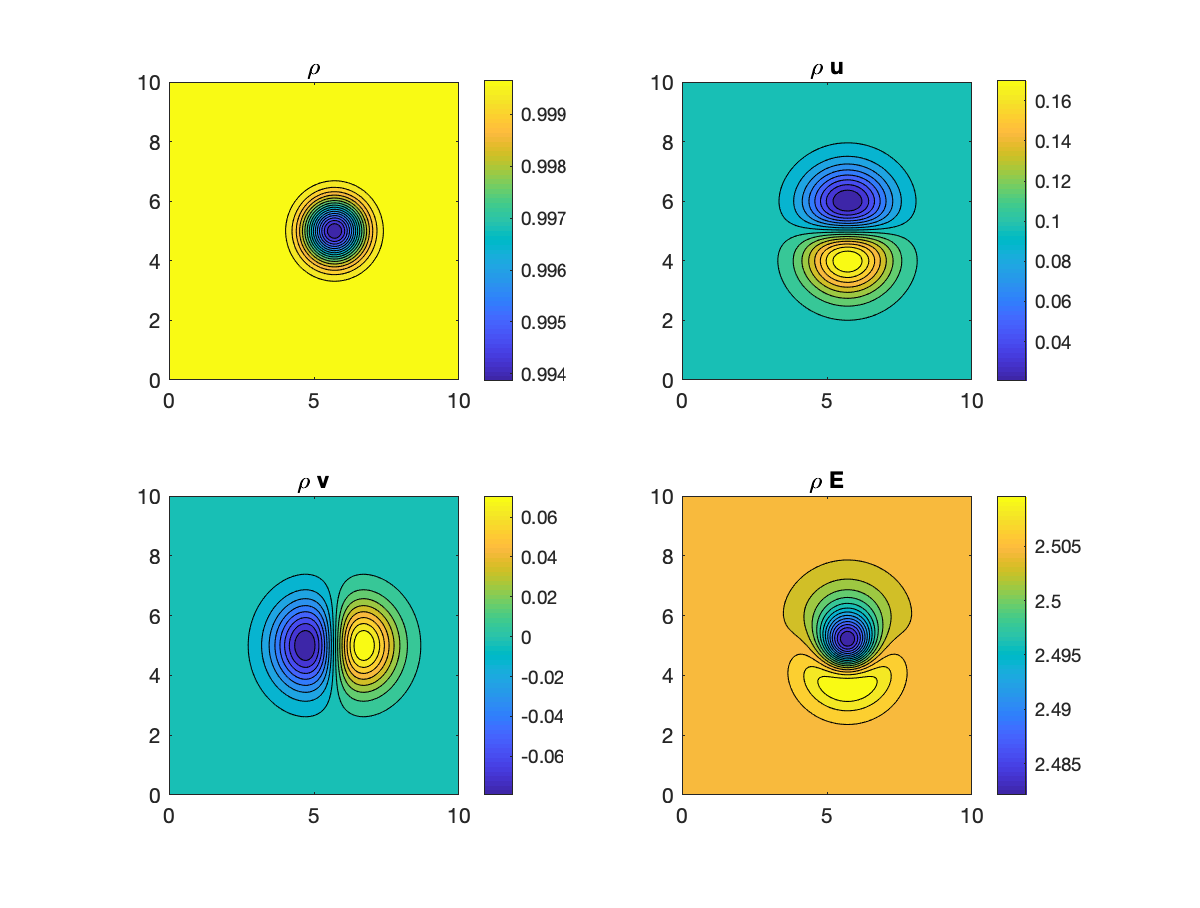
\includegraphics[width=1.0\textwidth]{final_sol_vortex.eps}


\indent \indent \indent \indent In all four solution components, at time $T = 5\sqrt{2}$.

\includegraphics[width=1.0\textwidth]{close-up.png}
\indent \indent \indent \indent A more close-up final solution, at time $T=5\sqrt{2}$.

\subsubsection{Error behaviors \& Filtering parameter $\alpha$}
Given the exact solution at all times and $x,y$, we can compute and compare our numerical errors, summarized in MATLAB console display on the current $\alpha$ choice, and step size. Here we take $l_{\infty}$ norm over the component-wise error $$
	E(i,j)=\vert f_{exact}(x_i,y_j) - \hat{f}(x_i,y_j)\vert_{\infty}
$$ where $\hat{f}$ is the numerical solution.

We loop over $\alpha \in \big[0.48,0.499\big]$ and all discretization choices $N \in \big[ 32, 64, 128\big]$.

    \begin{verbatim}
proj2_hongli
====================
current alpha: 0.48
current stepsize: 32
====================
rho error is: 5.1092e-05
rho u error is: 0.00093895
rho v error is: 0.00092598
rho E error is: 0.00041128
====================
total error is: 0.0023273
====================
====================
current alpha: 0.48
current stepsize: 64
====================
rho error is: 6.4255e-06
rho u error is: 0.00011283
rho v error is: 0.0001132
rho E error is: 5.2332e-05
====================
total error is: 0.00028479
====================
====================
current alpha: 0.48
current stepsize: 128
====================
rho error is: 7.8312e-07
rho u error is: 1.3915e-05
rho v error is: 5.605e-05
rho E error is: 6.5757e-06
====================
total error is: 7.7324e-05
====================
====================
current alpha: 0.499
current stepsize: 32
====================
rho error is: 1.1626e-05
rho u error is: 0.00014498
rho v error is: 0.00018249
rho E error is: 2.8349e-05
====================
total error is: 0.00036744
====================
====================
current alpha: 0.499
current stepsize: 64
====================
rho error is: 7.3792e-07
rho u error is: 1.0379e-05
rho v error is: 5.5984e-05
rho E error is: 2.8109e-06
====================
total error is: 6.9912e-05
====================
====================
current alpha: 0.499
current stepsize: 128
====================
rho error is: 6.2123e-08
rho u error is: 7.8958e-06
rho v error is: 5.6418e-05
rho E error is: 7.9143e-07
====================
total error is: 6.5168e-05
====================
\end{verbatim}

In order to ensure that the error behavior is overall fourth order, we compute the aggregate error as a reliable worst case upper bound over all solution components:
$$
	E_{total} = E_{\rho} + E_{\rho u} + E_{\rho v} + E_{\rho E}
$$

The error plot is shown below for different choice of $\alpha$ as we increase step size from $N=32,64,128$, on a $log-log$ scale. The benchmark $h^4$ means that we expect the method to be fourth order.

\begin{figure}[h]
\centering
\includegraphics[width=1.0\textwidth]{errors.png}
\caption{$L_{\infty}$ norm error behavior, over all solution components}
\end{figure}

\newpage
We see that the error behavior is roughly fourth order, and increasing our filtering parameter $\alpha$ will result in generally better error (the error plot in $\alpha = 0.499$ shifted downwards to $O(10^{-7}) \sim O(10^{-6})$). In order to confirm the exact order, we add a routine in computing and estimating the error slope by using MATLAB linear $polyfit$:

\begin{verbatim}
	using \alpha = 0.48, error is 3.0138 th order
	using \alpha = 0.499, error is 3.774 th order
\end{verbatim}

We can observe the conclusion that when $\alpha \rightarrow 0.5$, our compact filter

\noindent\underline{will provide numerical results asymptotically fourth-order}. By increasing $\alpha$ to be close to 0.5, we can obtain a fourth order scheme. 
\newpage
Indeed, as a side remark, if we increase even further to $\alpha=0.4999$, we get even closer to fourth-order accurate.
\begin{verbatim}
	using \alpha = 0.48, error is 3.0138 th order
	using \alpha = 0.4999, error is 3.8962 th order
\end{verbatim}

Another interesting observation is that there seems to be a discontinuity at $\alpha=0.5$, which would yield the following error behavior:
\begin{verbatim}
====================
current alpha: 0.5
current stepsize: 32
====================
rho error is: NaN
rho u error is: NaN
rho v error is: NaN
rho E error is: NaN
====================
total error is: NaN
====================
====================
current alpha: 0.5
current stepsize: 64
====================
rho error is: NaN
rho u error is: NaN
rho v error is: NaN
rho E error is: NaN
====================
total error is: NaN
====================
====================
current alpha: 0.5
current stepsize: 128
====================
rho error is: NaN
rho u error is: NaN
rho v error is: NaN
rho E error is: NaN
====================
total error is: NaN
====================
using \alpha = 0.48, error is 3.0138 th order
using \alpha = 0.5, error is NaN th order
\end{verbatim} 
meaning that there exists a limit to which we can filter our solution.

However, when $\alpha = 0.48$, the scheme will be less accurate and be 3rd order due to inherent oscillations.

\subsubsection{Kelvin-Helmholtz Instability}
Using our solver, we can simulate Kelvin-Helmholtz Instability at the final time $T = 1.0$ using $N=256$ steps for spatial discretization, which yields:
\begin{figure}[h]
\centering
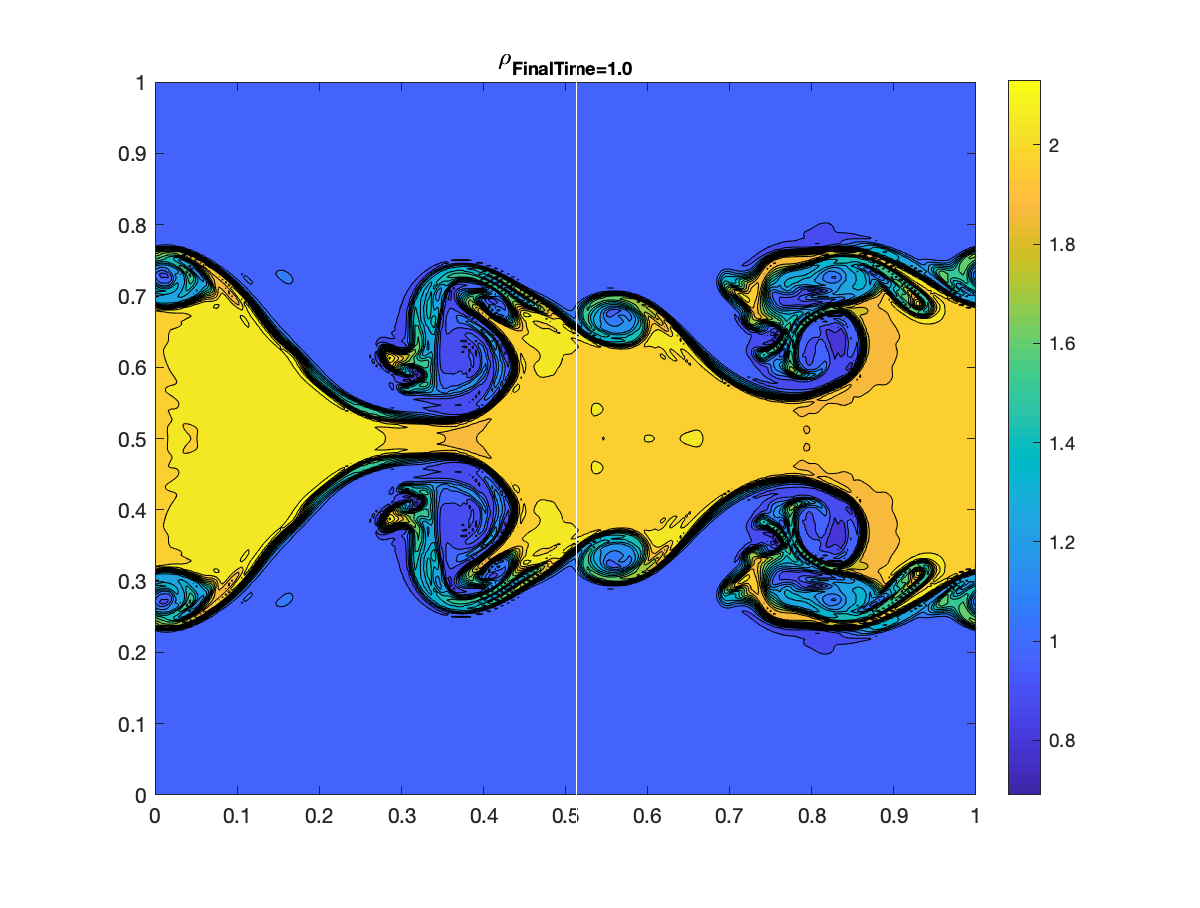
\includegraphics[width=1.0\textwidth]{kelvin_eps.eps}
\caption{Kelvin-Helmholtz Instability Simulation at $T=1.0$}
\end{figure}

In MATLAB, the routine roughly runs for 1 minute to obtain the numerical result.

The complete version of MATLAB code is as the following. Along with the individual runnable modules, the separate
\begin{verbatim}
utilities/
==========
compact_div.m
compact_filter.m
euler_fluxes.m
euler_rhs.m
euler_rk4step.m

numerical sol/
==========
vortex_convec.m // problem 1
kelvin.m // problem 2

\end{verbatim} 
files are also attached with the write-up.

Complete code below:
\begin{verbatim}
%  Math 228B, Hongli Zhao

%  Completed Project 2, solver for Euler's gas equations
%  u_t +div(F) = 0 with periodic boundary conditions
%  Divergence calculation using 4th order Padé scheme with filtering
%  Numerical integration using 4th order Runga-kutta scheme

% ============================================================
% function calls, organized by Proj2 spec
clear
% (f) Isentropic Vortex Convection problem
% and Kelvin-Helmholtz instability

% control sequences:
problem = 0; % 0 - vortex, 1 - kelvin
with_plot = 1; % turn with_plot = 1 to see final sol
see_error = 0; % turn see_error = 1 to see error plot

% load parameters given problem 0, 1
if problem == 0
    % vortex problem

    % define data holder for plotting
    % 2 (alpha choice) by 3 (step size choice)
    inf_err_data = zeros(2,3);
    inf_r_err_data = inf_err_data;
    inf_ru_err_data = inf_err_data;
    inf_rv_err_data = inf_err_data;
    inf_rE_err_data = inf_err_data;

    % change N for different results
    Ns = [32,64,128]; % N = 32,64,128
    alphas = [0.48,0.499];

    for alpha_idx=1:2 % over alpha
        for stpsz_idx=1:3 % over step size
            alpha = alphas(alpha_idx);
            % grid
            T = 5*sqrt(2);
            FinalTime = T;
            h = 10.0 / Ns(stpsz_idx);
            x = h * (0:Ns(stpsz_idx));
            y = h * (0:Ns(stpsz_idx));
            [x,y] = meshgrid(x,y);
            k = 0.3*h;
            adjust_factor = ceil(T/k);
            k = T/adjust_factor;
            % parameters
            gamma = 7/5; % gas constant
            b = 0.5; % vortex strength
            x_c = 5; y_c = 5;
            % initial solution
            d = sqrt((x - x_c).^2 + (y - y_c).^2);
            r = (1 - ((b^2)*(gamma-1)/(8*gamma*pi^2))...
                *exp(1-d.^2)).^(1/(gamma-1));
            p = r.^gamma;
            u = 0.1 - (0.5*b/pi)*exp(0.5*(1-d.^2)).*(y-y_c);
            v = (0.5*b/pi)*exp(0.5*(1-d.^2)).*(x-x_c);
            ru = r.*u;
            rv = r.*v;
            rE = p/(gamma-1) + r.*(u.^2 + v.^2)/2;

            % prepare exact solution
            u_inf = 0.1; v_inf = 0;
            r_inf = 1; p_inf = 1;
            x_exact = x_c + FinalTime*u_inf;
            d = sqrt((x-x_exact).^2 + (y-y_c).^2);
            r_exact = (1 -((gamma-1)*(b^2)/(8*gamma*pi^2))...
                *exp(1-d.^2)).^(1/(gamma-1));
            u_exact = u_inf - ((1/2)*b/pi)*exp((1/2)...
                *(1-d.^2)).*(y-y_c);
            v_exact = v_inf + ((1/2)*b/pi)*exp((1/2)...
                *(1-d.^2)).*(x-x_exact);
            p_exact = r_exact.^gamma;
            ru_exact = r_exact.*u_exact;
            rv_exact = r_exact.*v_exact;
            rE_exact = p_exact/(gamma-1)...
                +r_exact.*(u_exact.^2 + v_exact.^2)/2;

            %===================== Numerical sol
            for n = 1:adjust_factor
               [r,ru,rv,rE] = euler_rk4step(r,ru,rv,rE,h,k,alpha);
            end

            % Error matrices
            r_error_mat = r - r_exact;
            ru_error_mat = ru - ru_exact;
            rv_error_mat = rv - rv_exact;
            rE_error_mat = rE - rE_exact;
            % display info, comment out if wanted
            statement1 = ['current alpha: ', num2str(alpha)];
            statement2 = ['current stepsize: '...
                , num2str(Ns(stpsz_idx))];

            disp("====================");
            disp(statement1);
            disp(statement2);

            % calculate infinity norms for errors
            r_error = max(max(abs(r_error_mat)));
            ru_error = max(max(abs(ru_error_mat)));
            rv_error = max(max(abs(rv_error_mat)));
            rE_error = max(max(abs(rE_error_mat)));
            disp("====================");
            disp(['rho error is: ', num2str(r_error)]);
            disp(['rho u error is: ', num2str(ru_error)]);
            disp(['rho v error is: ', num2str(rv_error)]);
            disp(['rho E error is: ', num2str(rE_error)]);

            % overall error
            error_total = r_error+ru_error+rv_error+rE_error;
            disp("====================");
            disp(['total error is: ', num2str(error_total)]);
            disp("====================");
            inf_err_data(alpha_idx,stpsz_idx) = error_total;
            inf_r_err_data(alpha_idx,stpsz_idx) = r_error;
            inf_ru_err_data(alpha_idx,stpsz_idx) = ru_error;
            inf_rv_err_data(alpha_idx,stpsz_idx) = rv_error;
            inf_rE_err_data(alpha_idx,stpsz_idx) = rE_error;
        end
    end

    % populated inf_err_data, can plot
    if see_error == 1
        H = 10./Ns;
        error_data = zeros(size(inf_r_err_data));
        error_data(1,:) = 4 * inf_r_err_data(1,:);

        error_data(2,:) = 4 * inf_r_err_data(2,:);
        coe1 = polyfit(log(H),log(error_data(1,:)),1);
        slope1 = coe1(1);
        disp(['using \alpha = ',num2str(alphas(1)),...
            ', error is ',num2str(slope1),' th order'])
        coe2 = polyfit(log(H),log(error_data(2,:)),1);
        slope2 = coe2(1);
        disp(['using \alpha = ',num2str(alphas(2)),...
            ', error is ',num2str(slope2),' th order'])
        %============= granular plotting
        figure(1)
        subplot(1,2,1)
        loglog(H,H.^4,H,error_data(1,:),'LineWidth',2.5)

        title(['error behavior, \alpha=',num2str(alphas(1))])
        legend('h^4','agg err')
        subplot(1,2,2)
        loglog(H,H.^4,H,error_data(2,:),'LineWidth',2.5)
        title(['error behavior, \alpha=',num2str(alphas(2))])
        legend('h^4','agg err')
    end
else
    % kelvin problem
    N = 256;
    h = 1.0/N;
    x = (0:h:1.0); y = (0:h:1.0);
    T = 1.0;
    k = 0.3*h;
    adjust_factor = ceil(T/k); % factor to adjust k
    k = T/adjust_factor;
    [x,y] = meshgrid(x,y);
    gamma = 7/5; % gas constant
    % initial conditions
    r = zeros(size(x));
    domain1 = find(abs(y-0.5)<(0.15 + sin(2*pi*x)/200));
    domain2 = find(~(abs(y-0.5)<0.15 + sin(2*pi*x)/200));
    r(domain1) = 2;
    r(domain2) = 1;
    u = r-1;
    v = zeros(size(r));
    p = 3*ones(size(r));
    ru = r.*u;
    rv = r.*v;
    rE = p/(gamma-1)+r.*(u.^2 + v.^2)/2;
end

% time integration
% integrate in time for kelvin
if problem == 1
    alf = 0.480;
    for t = 0:k:T
        [r,ru,rv,rE] = euler_rk4step(r,ru,rv,rE,h,k,alf);
        figure(2)
        contourf(x,y,r,16)
        shading interp
        title('\rho_{FinalTime=1.0}')
        colorbar
    end
end

% plotting, with control 0 and 1
if with_plot ~= 0
    if problem == 0
        % see what happened
        figure(1)
        subplot(2,2,1)
        contourf(x,y,r,16)
        shading interp
        title('\rho')
        colorbar

        subplot(2,2,2)
        contourf(x,y,ru,16)
        shading interp
        title('\rho u')
        colorbar

        subplot(2,2,3)
        contourf(x,y,rv,16)
        shading interp
        title('\rho v')
        colorbar

        subplot(2,2,4)
        contourf(x,y,rE,16)
        shading interp
        title('\rho E')
        colorbar
    else
        figure(2)
        contourf(x,y,r,16)
        shading interp
        title('\rho_{FinalTime=1.0}')
        colorbar
    end
end


% ============================================================
% utilities

function divF = compact_div(Fx,Fy,h)
    % calculates the divergence of a grid function field
    % using the fourth order Padé method with periodic boundary
    % conditions

    % input:
    %   - Fx: (N+1)x(N+1) matrix; the flux function in the x-direction
    %   - Fy: (N+1)x(N+1) matrix; the flux function in the y-direction
    %   - h: grid spacing h

    % output:
    %   - divF: the matrix representing the divergence, for
    % a pair of components e.g. (rx,ry), it is a matrix resulted
    % from adding up two matrices.

    % preallocate matrices to store our divergence in each
    % component. In DX, we compute row-wise (y is fixed) and
    % similarly for DY.

    % ============================================================
    DX = zeros(size(Fx)); DY = zeros(size(Fy));
    n = length(DX)-1;
    % create coefficient matrix A, we solve Af' = (3/h)*f
    A = eye(n,n) * 4;
    for i=1:n-1
       A(i+1,i) = 1; % subdiag
       A(i,i+1) = 1; % superdiag
    end
    A(1,end) = 1; A(end,1) = 1;
    A = sparse(A); % sparsify

    % create rhs coefficient matrix B, and apply on data to
    % create b
    B = zeros(n,n);
    for i=1:n-1
       B(i+1,i) = -1; % subdiag
       B(i,i+1) = 1; % supdiag
    end
    B(1,end) = -1; B(end,1) = 1; % corner
    B = sparse(B); % make sparse

    f_data = Fx(1:n+1,1:n)';
    f_data = (3/h) * B * f_data;
    f_prime_data = A\f_data;
    DX(1:n+1,1:n) = f_prime_data';

    DX(:,end)=DX(:,1); % periodic


    f_data = Fy(1:n,1:n+1);
    f_data = (3/h) * B * f_data;
    f_prime_data = A\f_data;
    DY(1:n,1:n+1) = f_prime_data;


    DY(end,:)=DY(1,:); % periodic

    % add up to obtain divergence
    divF = DX + DY;
end



function [u] = compact_filter(u, alpha)
    % filters the numerical solution u

    % inputs:
    %   - u: our numerical solution, 4x(n+1)x(n+1) data
    % matrix storing values of r,ru,rv,rE defined on the x-y grid
    % when filtering, do for each component.

    %   - alpha: parameter

    % output:
    %   - u_new: the filtered smooth solution u computed using the
    % scheme, still a 4x(N+1)x(N+1) data matrix.
    % ======================================================
    size_u = size(u);
    n = size_u(3)-1;
    % compute parameters:
    a = (5/8) + (3*alpha)/4;
    b = alpha + 1/2;
    c = alpha/4 - 1/8;

    % tridiag matrix on lhs
    A = eye(n,n);
    for i=1:n-1
        A(i+1,i) = alpha; % subdiag
        A(i,i+1) = alpha; % superdiag
    end
    A(1,end) = alpha; A(end,1) = alpha;
    A = sparse(A); % sparsify
    % prepare right hand side in each loop
    rhs = zeros(n,n+1); % for all components
    for i = 1:4
        % first obtain data, which is (N+1)x(N+1)
        data = squeeze(u(i,:,:));
        % filter in x
        data(:,n+1) = data(:,1);

        % prepare right hand side
        % first take care of boundaries
        rhs(1,:) = (a*data(:,1)+(c/2)*(data(:,3)+data(:,n-1))...
            + (b/2)*(data(:,2)+data(:,n)))';
        rhs(2,:) = (a*data(:,2)+(c/2)*(data(:,4)+data(:,n))...
            + (b/2)*(data(:,3)+data(:,1)))';

        rhs(3:n-1,:) = (a*data(:,3:n-1)+...
            (c/2)*(data(:,5:n+1)+data(:,1:n-3))...
            + (b/2)*(data(:,4:n)+data(:,2:n-2)))';
        rhs(n,:) = (a*data(:,n)+(c/2)*(data(:,2)+data(:,n-2))...
            + (b/2)*(data(:,1)+data(:,n-1)))';

        % reassign boundary u(1)=u(N+1)
        data(:,1:n) = (A\rhs)';
        data(:,n+1) = data(:,1);

        % filter in y
        data(n+1,:) = data(1,:);
        data(:,n+1) = data(:,1);

        % prepare right hand side
        rhs(1,:) = a*data(1,:)+(c/2)*(data(3,:)+data(n-1,:))...
                + (b/2)*(data(2,:)+data(n,:));
        rhs(2,:) = a*data(2,:)+(c/2)*(data(4,:)+data(n,:))...
            + (b/2)*(data(3,:)+data(1,:));
        rhs(3:n-1,:) = a*data(3:n-1,:)+...
            (c/2)*(data(5:n+1,:)+data(1:n-3,:))...
                + (b/2)*(data(4:n,:)+data(2:n-2,:));
        rhs(n,:) = a*data(n,:)+(c/2)*(data(2,:)+data(n-2,:))...
                + (b/2)*(data(1,:)+data(n-1,:));

        % reassign boundary
        data(1:n,:) = A\rhs;
        data(n+1,:) = data(1,:);

        % put back filtered data
        u(i,:,:) = data;
    end
    % do four times, each time for one entry, we have 4x(N+1)x(N+1)
end





function [Frx,Fry,Frux,Fruy,Frvx,Frvy,FrEx,FrEy] = euler_fluxes(r, ...
    ru, rv, rE)
    % inputs: r, ru, rv, rE (vector components of u), each is a scalar
    % (written in general case so easily switched if needed)
    % outputs: flux functions of F, scalar, at (x,y)
    % ======================================================
    gamma = 7/5;
    u = ru./r;
    v = rv./r;
    p = (gamma-1)*(rE - (ru.*u + rv.*v)/2);
    Frx = ru;
    Fry = rv;
    Frux = ru.*u + p;
    Fruy = ru.*v;
    Frvx = Fruy;
    Frvy = rv.*v + p;
    FrEx = u.*(rE + p);
    FrEy = v.*(rE + p);
end




function [fr,fru,frv,frE] = euler_rhs(r, ru, rv, rE, h)
    % computes the right-hand side of the discretized divergence
    % there is a negative sign

    % inputs:
    %   - r, ru, rv, rE: input (N+1)x(N+1) matrices from which we
    % would like to calculate the divergence for
    %   - h: step size of your discretization, to be fed in when
    % approximating divergence

    % outputs:
    %   - fr, fru, fry, frE: the four divergence components
    % ======================================================

    % Get all 8 fluxes:
    [Frx,Fry,Frux,Fruy,Frvx,Frvy,FrEx,FrEy] = euler_fluxes(r, ...
    ru, rv, rE);

    fr = (-1) * compact_div(Frx,Fry,h);
    fru = (-1) * compact_div(Frux,Fruy,h);
    frv = (-1) * compact_div(Frvx,Frvy,h);
    frE = (-1) * compact_div(FrEx,FrEy,h);

end




function [r,ru,rv,rE] = euler_rk4step(r,ru,rv,rE,h,k,alpha)
    % calculate our final integrated solution
    % using 4th order accurate Runge-Kutta method
    % integrator in time t

    % inputs:
    %   - r, ru, rv, rE: the function values (at each (x,y) on grid)
    %   computed and organized in (N+1)x(N+1) matrices
    %   - h, alpha: parameters to feed into our compact filter
    %   - k: our time step, delta t

    % outputs:
    %   - r, ru, rv, rE: the function values evolved after 1 timestep

    % right hand side rhs is computed using euler_rhs
    % can consider as Ut = F(U), where U = [r,ru,rv,rE], F calcs div
    % ======================================================

    % ======= k1
    [fr1,fru1,frv1,frE1] = euler_rhs(r,ru,rv,rE,h);
    r_k1 = k * fr1; ru_k1 = k * fru1;
    rv_k1 = k * frv1; rE_k1 = k * frE1;

    % ======= k2
    [fr2,fru2,frv2,frE2] = ...
        euler_rhs(r + 0.5 * r_k1,ru + 0.5 * ru_k1, ...
            rv + 0.5 * rv_k1,rE + 0.5 * rE_k1,h);

    r_k2 = k * fr2; ru_k2 = k * fru2;
    rv_k2 = k * frv2; rE_k2 = k * frE2;
    % ======= k3
    [fr3,fru3,frv3,frE3] = ...
        euler_rhs(r + 0.5 * r_k2,ru + 0.5 * ru_k2, ...
            rv + 0.5 * rv_k2,rE + 0.5 * rE_k2,h);
    r_k3 = k * fr3; ru_k3 = k * fru3;
    rv_k3 = k * frv3; rE_k3 = k * frE3;
    % ======= k4
    [fr4,fru4,frv4,frE4] = ...
        euler_rhs(r + r_k3,ru + ru_k3, ...
            rv + rv_k3,rE + rE_k3,h);
    r_k4 = k * fr4; ru_k4 = k * fru4;
    rv_k4 = k * frv4; rE_k4 = k * frE4;

    % weighted average
    r_raw = r + (1/6) * (r_k1 + 2*r_k2 + 2*r_k3 + r_k4);
    ru_raw = ru + (1/6) * (ru_k1 + 2*ru_k2 + 2*ru_k3 + ru_k4);
    rv_raw = rv + (1/6) * (rv_k1 + 2*rv_k2 + 2*rv_k3 + rv_k4);
    rE_raw = rE + (1/6) * (rE_k1 + 2*rE_k2 + 2*rE_k3 + rE_k4);

    % in order to use compact_filter, need to assemble into u_raw
    size_u = [4, size(r)];
    u_raw = zeros(size_u);

    u_raw(1,:,:) = r_raw;
    u_raw(2,:,:) = ru_raw;
    u_raw(3,:,:) = rv_raw;
    u_raw(4,:,:) = rE_raw;

    % filter our solution in each component
    % returns a 4x(n+1)x(n+1) matrix to dessemble
    u_clean = compact_filter(u_raw,alpha);

    % dessemble into our output
    r = reshape(u_clean(1,:,:),size(r));
    ru = reshape(u_clean(2,:,:),size(ru));
    rv = reshape(u_clean(3,:,:),size(rv));
    rE = reshape(u_clean(4,:,:),size(rE));
end
\end{verbatim}

        \color{gray} 
\begin{verbatim}
====================
Display numerical results...
current alpha: 0.48
current stepsize: 32
====================
rho error is: 5.1092e-05
rho u error is: 0.00093895
rho v error is: 0.00092598
rho E error is: 0.00041128
====================
total error is: 0.0023273
====================
====================
current alpha: 0.48
current stepsize: 64
====================
rho error is: 6.4255e-06
rho u error is: 0.00011283
rho v error is: 0.0001132
rho E error is: 5.2332e-05
====================
total error is: 0.00028479
====================
====================
current alpha: 0.48
current stepsize: 128
====================
rho error is: 7.8312e-07
rho u error is: 1.3915e-05
rho v error is: 5.605e-05
rho E error is: 6.5757e-06
====================
total error is: 7.7324e-05
====================
====================
current alpha: 0.499
current stepsize: 32
====================
rho error is: 1.1626e-05
rho u error is: 0.00014498
rho v error is: 0.00018249
rho E error is: 2.8349e-05
====================
total error is: 0.00036744
====================
====================
current alpha: 0.499
current stepsize: 64
====================
rho error is: 7.3792e-07
rho u error is: 1.0379e-05
rho v error is: 5.5984e-05
rho E error is: 2.8109e-06
====================
total error is: 6.9912e-05
====================
====================
current alpha: 0.499
current stepsize: 128
====================
rho error is: 6.2123e-08
rho u error is: 7.8958e-06
rho v error is: 5.6418e-05
rho E error is: 7.9143e-07
====================
total error is: 6.5168e-05
====================
\end{verbatim} \color{black}

%==========
\end{document}